% *********************************************************************
% © 2021–2024 Jeremy Sylvestre
%
% Permission is granted to copy, distribute and/or modify this document
% under the terms of the GNU Free Documentation License, Version 1.3 or
% any later version published by the Free Software Foundation; with no
% Invariant Sections, no Front-Cover Texts, and no Back-Cover Texts. A
% copy of the license is included in the appendix entitled “GNU Free
% Documentation License” that appears in the output document of this
% PreTeXt source code. All trademarks™ are the registered® marks of
% their respective owners.
%
% *********************************************************************

\newcommand*{\xmin}{1}
\newcommand*{\xmax}{5.25}
\newcommand*{\ymin}{-5}
\newcommand*{\ymax}{5}
\newcommand*{\func}{\x * \x * \x - 9 * \x * \x + 23 * \x - 14}

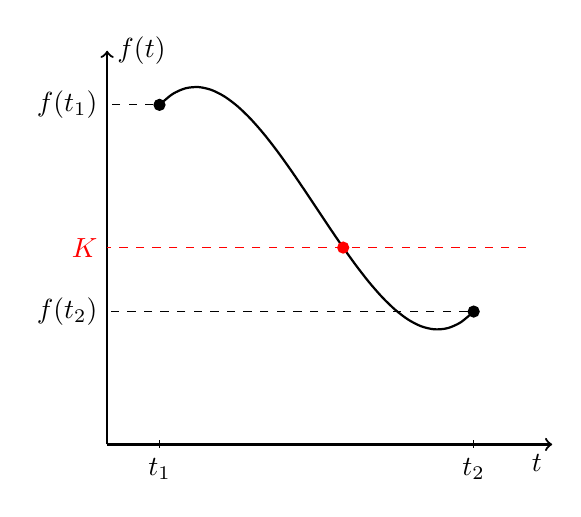
\begin{tikzpicture}
[
	closedpt/.style={circle,draw,fill,inner sep=0pt,minimum size=4pt},
	openpt/.style={circle,draw,inner sep=0pt,minimum size=4pt},
	xscale=1.33,
	yscale=0.5
]

	% example graph
	\draw[thick, domain=1.5:4.5, smooth] plot (\x,{\func});

	\node[closedpt] (top) at (1.5,3.625) {};
	\draw (1.5,-4.9) -- (1.5,-5.1) node[below] {$t_1$};
	\draw[dashed] (top) -- (\xmin,3.625) node[left] {$f(t_1)$};
	\node[closedpt] (bottom) at (4.5,-1.625) {};
	\draw (4.5,-4.9) to (4.5,-5.1) node[below] {$t_2$};
	\draw[dashed] (bottom) to (\xmin,-1.625) node[left] {$f(t_2)$};

	% axes
	\draw[->,thick] (\xmin,\ymin) -- (\xmax,\ymin) node[below left] {$t$};
	\draw[->,thick] (\xmin,\ymin) -- (\xmin,\ymax) node[right] {$f(t)$};

	\draw[dashed,red] (5,0) -- (\xmin,0) node[left] {$K$};
	\node[closedpt,red] at (3.254,0) {};

\end{tikzpicture}
